\subsection{Обзор существующих аналогов}
\label{sec:analysis:analogues}

Процесс управления категориями является ключевым в построении взаимодействия между пользователем и ботом. Для удобного и быстрого управление домашней бухгалтерией, требуется средство с интуитивно понятным интерфейсом.

В данном разделе представлены два самых популярных представителя ботов для контроля за персональными расходами: Greenz Bot и \linebreak WhereIsMyMoney Bot. Для каждого из аналогов будет даваться краткая характеристика, примеры работы, а также преимущества и недостатки данных программных продуктов.

\subsubsection{} Greenz Bot
\label{sec:analysis:analogues:greenz}

Бот обладает широким спектром функциональности, включая синхронизацию с Google таблицами, установку желаемой суммы, которую пользователь не хочет превышать в месяц. Использование бота предполагает написание пользователем категории и суммы, а также, если необходимо, указание даты и подкатегории. Принцип работы показан на рисунке \ref{fig:analysis:analogues:greenz}.

Возможность просмотра баланса отображена на рисунке \ref{fig:analysis:analogues:greenz_balance}.

Достоинства Greenz Bot:

\begin{itemize}
	\item Поддержка человеческого языка. Бот способен распознавать запросы пользователя, которые представляют собой предложения, сокращения и так далее. К примеру, командой <<бенз 150>>, пользователь добавит -150 единиц валюты в категорию Автомобиль.
	\item Возможность синхронизации с Google таблицами.
	\item Установка желаемой суммы, которую пользователь не хочет превышать за месяц.
\end{itemize}

Из минусов приложения можно выделить отсутствие следующих возможностей:

\begin{itemize}
	\item создание собственной категории;
	\item указание валюты.
\end{itemize}

\begin{figure}[!h]
	\centering
	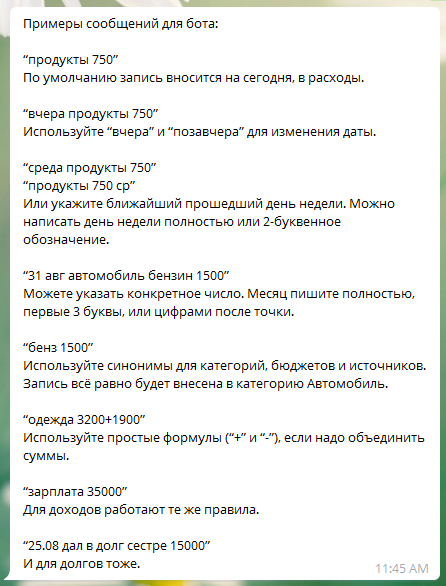
\includegraphics[scale=0.7]{greenzbot.png} 
	\caption{Принцип работы Greenz Bot}
	\label{fig:analysis:analogues:greenz}
\end{figure}

\subsubsection{} WhereIsMyMoneyBot
\label{sec:analysis:analogues:whereismymoney}

Телеграм-бот WhereIsMyMoneyBot является хорошим помощником \linebreak для людей, желающих видеть, куда уходят их деньги. Бот поддерживает английский и русский языки, что помогает привлечь больше аудитории. Принцип работы бота описан на рисунке \ref{fig:analysis:analogues:whereismymoneybot}.

Приложение работает следующим образом: пользователь вводит сумму, которую потратил, а также категорию, состоящую из одного слова. Бот создает новую категорию и записывает в нее операцию.

Предлагается подробная история операций по категориям, а также, после каждого добавления операции предлагает статистику по количеству денег, потраченных на товары этой категории, всего потраченных денег в этом месяце, также сегодня. Помимо всего этого, можно настроить ежемесячные или еженедельные уведомления, что, безусловно, является большим преимуществом.

Достоинствами WhereIsMyMoneyBot являются:

\begin{itemize}
	\item возможность создания категорий;
	\item поддержка нескольких языков;
	\item наличие уведомлений.
\end{itemize}

\begin{figure}[!h]
	\centering
	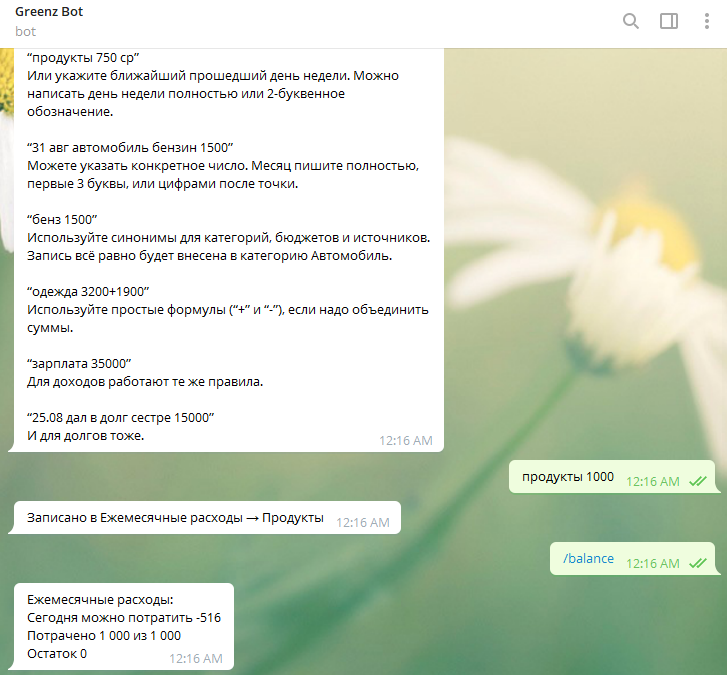
\includegraphics[scale=0.5]{greenzbot_balance.png} 
	\caption{Просмотр баланса в Greenz Bot}
	\label{fig:analysis:analogues:greenz_balance}
\end{figure}

\begin{figure}[!h]
	\centering
	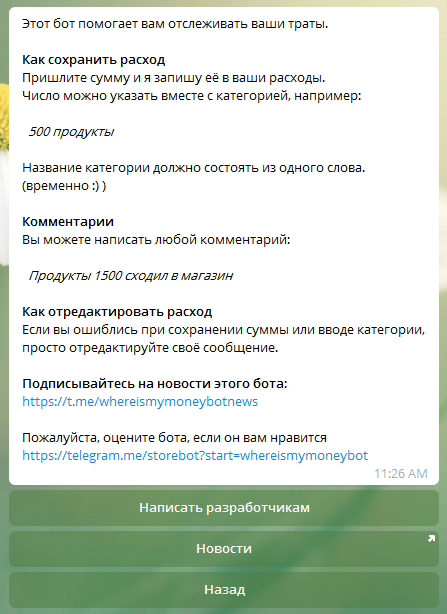
\includegraphics[scale=0.7]{whereismymoneybot.png} 
	\caption{Принцип работы WhereIsMyMoneyBot}
	\label{fig:analysis:analogues:whereismymoneybot}
\end{figure}

Из минусов приложения можно выделить отсутствие следующих возможностей:

\begin{itemize}
	\item изменение категории;
	\item указание валюты.
\end{itemize}

После обзора аналогов был сделан вывод о том, что современные финансовые боты учитывают доходы, расходы, позволяют экспортировать статистику в различных форматах данных. Недостатками же является отсутствие возможности создания собственных категорий, а также отсутствие валюты.

В проектируемом программном средстве планируется использовать все достоинства существующих на рынке ботов, а также исправление их недостатков.


